\chapter{TINJAUAN PUSTAKA}

% Ubah konten-konten berikut sesuai dengan isi dari tinjauan pustaka
\section{Hasil Penelitian Terdahulu}

\subsection{\emph{Vehicle Re-Identification System Based on Appearance Features}}
Pada tahun 2021, Dawei Xu bersama lima rekannya membuat penelitian yang berjudul "Vehicle Re-Identification System Based on Appearance Features" \cite{Xu2022}. Pada penelitian tersebut, Dawei Xu bersama lima rekannya mengusulkan metode re-identifikasi kendaraan dengan ekstrasi fitur jaringan multicabang dan fitur pengambilan dua tahap. Pengambilan dua tahap tersebut diantaranya adalah menambahkan parameter karakteristik dan penampilan kendaraan termasuk warna dan model kendaraan. Adapun dataset yang digunakan pada penelitian tersebut adalah Veri-776 dan VehicleID. Setelah melakukan penelitian menggunakan dataset dan algoritma yang sudah dibuat, mAP meningkat sebesar 2,43\% dan 2,7\% pada dua dataset yang digunakan, Rank-1 meningkat sebesar 1,85\% dan 2,9\%, dan Rank-5 meningkat sebesar 0,84\% dan 0,8\%.

\subsection{\emph{Vehicle Re-identification in Aerial Imagery : Dataset and Approach}}
Berdasarkan paper yang berjudul ”Vehicle Re-identification in Aerial Imagery: Dataset and Approach”, Peng Wang bersama lima rekannya membuat dataset untuk reidentifikasi kendaraan dengan mengaplikasikan \emph{Unmanned Aerial Vehicle} (UAV) sebagai alat pengambil citra \cite{Wang2019vehicle}. Pengaplikasian UAV telah menarik banyak perhatian baik dari sektor industri maupun akademisi. Namun, identifikasi ulang kendaraan berbasis UAV masih jarang dipelajari, meskipun memiliki banyak potensi seperti pelacakan jangka panjang, pengambilan objek visual, dan lain lain. Salah satu alasannya adalah kurangnya dataset terkait yang tersedia untuk umum. Oleh karena itu, Peng Wang bersama lima rekannya mengumpulkan dan merilis dataset VRAI (Vehicle Re-identification in Aerial Imagery) yang terdiri dari 137.613 gambar dari 13.022 sampel kendaraan.

\section{Dasar Teori}

\subsection{Reidentifikasi Mobil}

Pada dunia visi komputer, reidentifikasi adalah proses mencocokkan dua atau lebih citra suatu obyek berdasarkan identitasnya. sistem reidentifikasi yang umum dipelajari oleh para peniliti biasanya adalah sistem reidentifikasi orang dan mobil. Sebagai contoh pada sistem reidentifikasi mobil, identitas yang dicocokkan adalah warna mobil, model mobil, bumper, bentuk atap, velg ban, dan lain-lain. Dengan memanfaatkan visi komputer, proses reidentifikasi mobil dapat dilakukan secara otomatis. Sistem reidentifikas mobil bekerja dengan cara mengambil citra mobil di beberapa kamera di bawah perspektif pemantauan tertentu. Citra tersebut lalu diproses oleh sistem yang mengekstrak fitur dan mencocokkannya untuk menentukan apakah citra mobil yang diberikan adalah mobil yang sama.

\subsection{\emph{Unmanned Aerial Vehicle}}

\emph{Unmanned Aerial Vehicle} (UAV) merupakan jenis pesawat terbang yang dikendalikan alat sistem kendali jarak jauh lewat gelombang radio. \emph{Unmanned Aerial Vehicle} (UAV) merupakan sistem tanpa awak (\emph{Unmanned System}) yaitu sistem berbasis elektro mekanik yang dapat melakukan misimisi terprogram dengan karakteristik sebuah mesin terbang yang berfungsi dengan kendali jarak jauh oleh pilot atau mampu mengendalikan dirinya sendiri, menggunakan hukum aerodinamika untuk mengangkat dirinya sendiri \cite{UAV1}. \emph{Unmanned Aerial Vehicle} (UAV) mempunyai berbagai macam jenis ukuran, bentuk, dan fungsi \cite{UAV2}. Bahan material dari \emph{Unmanned Aerial Vehicle} (UAV) terbuat dari bahan yang ringan, sehingga bisa terbang dengan cepat dan terbang pada ketinggian yang rendah maupun ketinggian tertentu. \emph{Unmanned Aerial Vehicle} (UAV) sendiri memiliki kamera, infra merah, GPS, sensor, dan alat pendukung lainnya.

Saat ini masyarakat luas sudah mulai memanfaatkan \emph{Unmanned Aerial Vehicle} (UAV) untuk urusan hobi maupun militer. Salah satu contohnya adalah di dunia fotografi dan vidiografi. Para pegiat fotografi dan vidiografi profesional biasanya memiliki \emph{Unmanned Aerial Vehicle} (UAV) yang berukuran kecil dan ringan untuk memotret dan merekam objek dari ketinggian. Hal tersebut juga dilakukan oleh para peneliti khususnya di bidang visi komputer. Pemanfaatan \emph{Unmanned Aerial Vehicle} (UAV) oleh para peneliti digunakan sebagai alat pengambil citra untuk mebuat sebuah dataset. \emph{Unmanned Aerial Vehicle} (UAV) dapat menjangkau lokasi-lokasi yang sulit terjangkau oleh manusia. Selain itu, sudut tangkap kamera juga akan lebih variatif dengan memanfaatkan \emph{Unmanned Aerial Vehicle} (UAV).

\subsection{\emph{Deep Learning}}

\begin{figure} [ht] \centering
  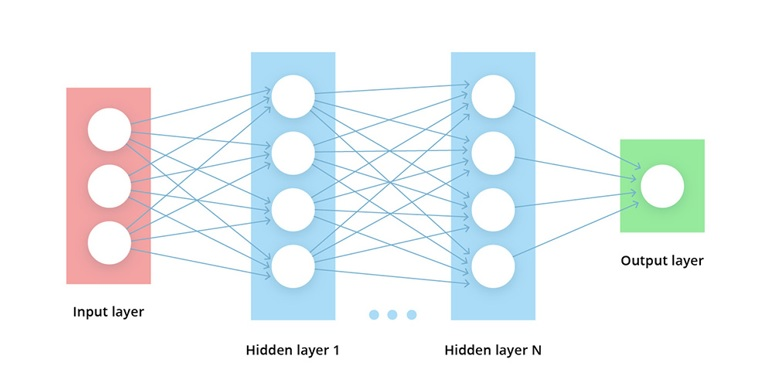
\includegraphics[scale=0.75]{gambar/deep-learning.jpg}
  \caption{\emph{Deep Learning 4 Layer} \cite{GambarDeepLearning}}
  \label{fig:DeepLearning4Layer}
\end{figure}

\emph{Deep learning} merupakan salah satu cabang dari \emph{machine learning}. \emph{Deep learning} juga merupakan salah satu algoritma dari \emph{Artificial Neural Network} yang terinspirasi dari sistem otak manusia. Algoritma pada \emph{deep learning} mempunyai kemampuan yang unik, yaitu dapat mengekstraksi fitur secara otomatis. Lapisan tersembunyi (\emph{hidden layer}) pada \emph{deep learning} lebih banyak daripada \emph{Artificial Neural Network}, sehingga pada \emph{Artificial Neural Network} membutuhkan lebih banyak informasi tentang data masukan untuk menentukan model yang cocok. Berbeda dengan \emph{deep learning} yang tidak membutuhkan informasi apapun terhadap data yang akan dipelajarinya karena secara mandiri dapat memilih model yang optimal. Beberapa contoh dari \emph{deep learning} adalah \emph{Deep Neural Network} (DNN), \emph{Recurrent Neural Network} (RNN), dan \emph{Convolutional Neural Network} (CNN). \cite{DeepLearningJWGPutra}

\subsection{\emph{Convolutional Neural Network}}

\emph{Convolutional Neural Network} (CNN) adalah salah satu jenis \emph{neural network} yang biasa digunakan pada data citra. CNN bisa digunakan untuk mendeteksi dan mengenali objek pada sebuah citra \cite{CNNQolbiyatulLina}. Secara garis besar CNN tidak jauh beda dengan \emph{neural network} lainnya. CNN terdiri dari neuron yang memiliki \emph{weight, bias} dan \emph{activation function}. \emph{Convolutional layer} juga terdiri dari neuron yang tersusun sedemikian rupa sehingga membentuk sebuah filter dengan panjang dan tinggi (\emph{pixels}).

\begin{figure} [ht] \centering
  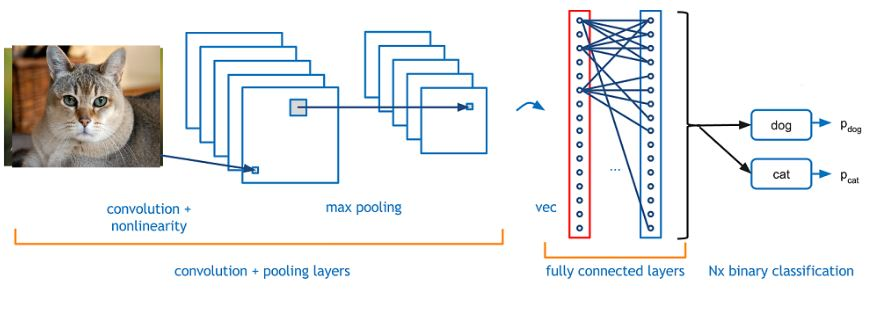
\includegraphics[scale=0.75]{gambar/cnn.jpg}
  \caption{\emph{Convolutional Neural Network} \cite{GambarCNN}}
  \label{fig:ConvolutionalNeuralNetwork}
\end{figure}

Seperti pada gambar \ref{fig:ConvolutionalNeuralNetwork}, CNN terbagi menjadi 3 \emph{layer} utama. \emph{Layer} pertama adalah \emph{convolution layer}, yang kedua adalah \emph{pooling layers}, dan terakhir adalah \emph{fully connected layers}. Berbagai jenis \emph{layer} tersebut mempunyai peran yang berbeda. \emph{Convolutional layer} digunakan untuk mengekstrasi fitur data yang akan digunakan untuk \emph{training}. Selanjutnya \emph{pooling layer} digunakan untuk membuat \emph{filter} baru berdasarkan aturan yang diinginkan (biasanya antara membuat \emph{filter} dari nilai maksimal atau membuat \emph{filter} menggunakan nilai rata-rata). :ayer yang terakhir adalah \emph{fully connected layer}. \emph{Layer} ini sebenarnya adalah MLP (\emph{multilayer perceptron}) yang merupakan bagian dari \emph{artificial neural network} dan terdiri dari sejumlah neuron yang dihubungkan oleh bobot-bobot penghubung. Neuron ini disusun dalam lapisan yang terdiri dari satu lapisan input (\emph{input layer}), satu atau lebih lapisan tersembunyi (\emph{hidden layer}), dan satu lapisan output (\emph{output layer}). Lapisan \emph{input} menerima sinyal dari luar, kemudian melewatkannya ke lapisan tersembunyi pertama, yang akan diteruskan sehingga akhirnya mencapai lapisan \emph{output}. \cite{CNN}